\documentclass[../main.tex]{subfiles}
\providecommand{\main}{..}
%\biblio
%\addbibresource{\main/main.bib}

\begin{document}

After loading the data into in Ipython notebook, I first removed data from
impossible dates from Actions.csv, and then I checked all of the data for
duplicate entries or other errors. Since we are interested in the amount of
money donated by people, I figured that we should account for inflation and
price changes, so I downloaded CPI data from the St. Louis Federal Reserve
Bank and used it to add an additional number, the value of the gift in
1982-1984 dollars, to each recorded instance of a gift. I then created various hash
tables with the given information. I created a hash table containing each
person's given biographical information so demographics can be analyzed. 
I created the hash tables events history,
gift history, and actions history where the key is an identification number
of a person, and the value is the kind of history associated with that
dictionary and person. These tables can be used to create time series data
for individuals about their donations and event attendance; however, I used
them simply to compute $y_i$ the number of years each person $i$ was in the data and
the number of posthumous donors. We computed $y_i$ by finding the difference
between the date of the first form of contact, an action, event, or
donation, and either the death date or the date the actions file stopped
being recorded. This value is recorded as a floating point by uniformly at
random choosing the death month of deceased people under the assumption that
people die randomly throughout the year. The value is also computed in such
a way that if person $i$ is in the data for less than a year, we let $i = 1$
because these people would probably not donate much more anyway, and
dividing by small fractions can really overstate how much people would have
donated yearly and cause crazy outliers.

After having created these histories, I
then created hash tables event count, action count, and gift count. The
values of event count are the total number of events a person has attended;
the value of actions count are $[a_i, b_i, c_i, d_i]$ where $a_i$ is the
number of time person $i$ has been emailed, $b_i$ is the number of time
person $i$ has been called, $c_i$ is the number of times person $i$ has had
a meeting, and $d_i$ is the number of times person $i$ has been mailed; and
the values of gift count are $[e_i, f_i, g_i]$ where $e_i$ and $f_i$ are the
total nominal and real amounts donated by person $i$ and $g_i$ is the number
of times person $i$ donated.

After having created all of these connected hash tables, we could easily
compute various metrics. The objective is to cluster by amount donated and
how the person was contacted and see if there are any differences among
clusters that provide some insight about how to alter actions of the Office
of Advancement. Since people enter the data on different years, and leave
the data on different years, we computed $\dfrac{e_i}{y_i}$,
$\dfrac{f_i}{y_i}$, and $\dfrac{g_i}{y_i}$ for $i$ in gift count as measures
of donations and the average number of times a person is contacted per year
as a measure of actions. In addition to this measurement, for each person we
found what percentage of total types of contact fell into each category. For
each person I created a seven dimensional vector and clustered over these all
of these excluding $\dfrac{e_i}{y_i}$.

Clustering was done many times and a bit of outlier filtering was done.
There are 16686 individuals in these files since the start of Actions.csv,
and because we were measuring percentages of contact, we decided to filter
out people who have had 3 or less contacts because they cause a bunch of
weird percentages that have a large influence on the clustering algorithm.
After filtering these people out, we have 2231 people left, and then
removing posthumous donators from that group leaves 2143 people. We
initially clustered over these people, making sure to run the elbow graph
analysis multiple times. When doing this we noticed that someones we would
get a standard looking elbow graph with the elbow at four, but other times we would an elbow graph
with kinks in it with the first kink at four, like the one below.

Fourth elbow graph including outliers:

\vspace{1mm}

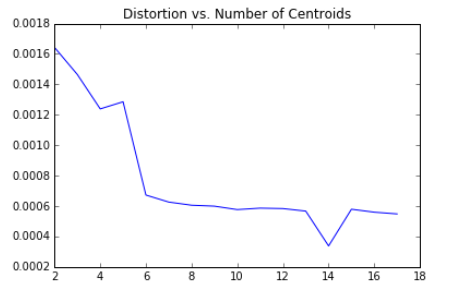
\includegraphics[width=10cm, height=8cm]{cluster1_elbow4.png}

Literature says that kinks in these graphs can be cause by extreme outliers
\cite{elbow1}. We performed PCA analysis in two and three dimensions, and
indeed there seemed to be a few extreme outliers. The most variation of the factors clustered over is present
in the amount donated per year. There six individuals from this original
clustering that donated absolutely staggering amounts of money, which was
throwing our analysis off. We removed these people and reclustered. Our
elbow graphs looked a lot less kinky. When choosing the number of clusters
here, one should choose the number of clusters right before the first kink
occurs, so long as a certain amount of variation is explained \cite{elbow1}.
Based on this, we chose to create five clusters.
Below is a three dimensional PCA analysis of the final clusterings, to give
a visual idea of how good the clusters are.

\vspace{1mm}

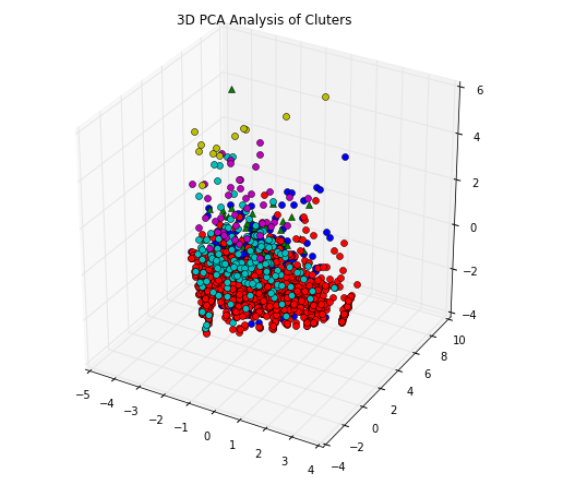
\includegraphics[width=10cm, height=8cm]{cluster2_3D_pca.png}

\end{document}
